\section{Data selection}
\label{sec:dsphi:sel}

The data sample used in this analysis amounts to
$1\invfb$ of $pp$ collisions at $7\tev$ collected by the \lhcb detector in 2011.
Events are selected by the trigger at hardware level if they fulfill the requirements of the \lone
hadron trigger, or any track in the event fulfills any \lone trigger line requirement (\tis).
Further trigger requirements are applied at the \hlttwo level, where events are required to pass at
least one of the hadronic topological triggers (see \Sec{sec:lhcb:trig} for more details) with
\tos.

The \Ds meson is only reconstructed from the Cabibbo favoured decay \dstokkpi,
which has a branching fraction of $(5.39\pm0.21)\e{-2}$.
Furthermore, the mass of the reconstructed particle must fall within $25\mev$ of
$m_{\Ds}^\pdg=1968.30\pm0.11\mev$; where the superscript \pdg indicates the nominal mass of the
indicated particle from \Ref{PDG2012}.
The \Ds meson decays weakly, and therefore has a non-zero lifetime,
$\tau_{\Ds}=(5.00\pm0.07)\e{-13}\sec$, and thus an extremely narrow width, so the value of $25\mev$
is primarily to account for detector resolution effects.
In order for the candidate to have the correct decay topology, it is also required that the \Ds
vertex lies downstream of the \Bp decay vertex.

Candidate \phii mesons are reconstructed from the decay mode \phitokk, where
$\BF(\phitokk)=(0.498\pm0.005)$ and are accepted if the
invariant \kk mass, $\mass{\kk}$, is within $40\mev$ of
$\mass{\phi}^\pdg=(1019.461\pm0.019)\mev$~\cite{PDG2012}.
The \phii meson decays strongly, and therefore has an appreciable width,
$\Gamma_\phi=(4.266\pm0.031)\mev$, but the detector resolution is better for the \phii than the \Ds
because it has zero lifetime.
Therefore, a mass window of $40\mev$ is extremely wide; but further mass constraints of the \phii
are applied in the fit used to obtain the signal yield: a signal region is defined by a window that
extends only $20\mev$ from $\mass{\phi}^\pdg$, and a sideband region

All tracks forming the candidate mesons must fulfill requirements on the transverse momentum,
$\pt>100\mev$, and tracks from the \Ds(\phii), $p>1(2)\gev$.
Geometrical constraints are also placed on the tracks.
One important geometrical variable is the \gls{IP}, which is defined as the perpendicular distance
between the vertex in question and the line of flight of a particle.
The \chisq per degree of freedom of the track fit, $\chisqtrk/\ndof$, must be less than four.
%and
%$\min\left(\chisqip\right)>4$.
The variable \chisqip is defined as the increase in the \chisq of the vertex fit (\chisqvtx) when
the signal track is combined with the \pv; the $\min\left(\chisqip\right)$ is the minimum \chisqip
with respect to all \glspl{PV}, this selection requires $\min\left(\chisqip\right)>4$.
Loose \pid requirements are also placed on all tracks, and further \pid constraints are applied in
the \bdt, which is detailed later.


The \Bp vertex fit is performed by constraining the mass of the \Ds candidate to its known
mass~\cite{PDG2012}, and requirement a \chisqvtx per degree of freedom of
less than ten.
%A requirement of $\cos\thetadir>0.999$ must also be met.
The angle between the momentum vector of the \Bp candidate and
the vector formed by the \pv and decay vertex of the \Bp is known as the direction angle,
\thetadir.
Were the resolution of the \lhcb detector to be perfect, a real decay would have $\cos\thetadir=1$,
here $\cos\thetadir$ must be greater than 0.999.
Prompt background from the \pv is suppressed by requiring that the lifetime of the \Bp,
$\tau_{\Bp}$, is greater than $0.2\ps$.
A cut on the \DOCA is applied to the \Ds candidate; where the \DOCA is defined as the maximum
distance of closest approach between all pairs of daughter particles.
%To ensure that the
Selection criteria are summarized in \Tab{tab:dsphi:sel}.

%Candidate \Ds and \phii mesons are reconstructed only in the decays \decay{\Ds}{\kkpi} and
%\phitokk, where the \Ds decay is the Cabibbo favoured mode.
%Each daughter track has a $\chisqtrk/\ndof<4$, a \pt of at least $100\mev$, and a minimum momentum
%of $1$ or $2\gev$ for tracks originating from the \Ds and \phii, respectively.
%Each track in the event must also be detached from the \pv, and are only accepted if the
%$\chisqvtx/\ndof$ increases by more than four when the track is used in the vertex fit, compared to
%when it is omitted.
%Very loose PID requirements are also placed on the tracks, this is more to reduce the rate of the
%stripping line that to identify pions and kaons, this is done later in the selection process.

%The \Ds and \phii are also subject to requirements on the \chisq of the vertex separation,
%\chisqvs, which is tighter for the \Ds because of its finite lifetime.
%Full stripping requirements are given in \Tab{tab:dsphi:sel}.

\begin{table}[!ht]
  \caption[Selection requirements of \btodsphi candidates]
  {
    Selection applied to the \btodsphi candidates.
    %The DOCA variable is defined as the maximum distance of closest approach between all pairs of
    %all pairs of daughter particles.
    %All remaining variables are defined in the text.
  }
  \label{tab:dsphi:sel}
  \begin{center}
    \begin{tabularcuts}
      \Bp
      %\multirow{5}{*}{\Bp}
       & $\sum p_T^\mathrm{tracks}$ &$>$& $5$ & GeV \\
      & \chisqvtx/\ndof &$<$& 10 \\
      & \chisqip &$<$& 25 \\
      & $\tau$ &$>$& $0.2$ & ps \\
      & $\cos\thetadir$ &$>$& $0.999$ \\
      \littlerule
      \Ds
      %\multirow{3}{*}{\Ds}
      & $\sum p_T^\mathrm{tracks}$ &$>$& $1.8$ & GeV \\
      & \chisqvtx/\ndof &$<$& 10 \\
      & \DOCA &$<$& $0.5$ & mm \\
      \littlerule
      Tracks from \Ds
      %\multirow{6}{*}{Tracks from \Ds}
      & \pt &$>$& $100$ & MeV \\
      & $p$ &$>$& $1$  & GeV\\
      & $\chisqtrk/\ndof$ &$<$& $4$ \\
      & $\min\!\left(\chisqip\right)$ &$>$& $4$ \\
      & \chisqfd &$>$& 36 \\
      & $\dllkpi(K)$ &$>$& $-10$ \\
      & $\dllkpi(\pi)$ &$<$& $20$ \\
      \littlerule
      \phii
      %\multirow{2}{*}{$\phi$}
      & $\sum\pt^\mathrm{tracks}$ &$>$& 1&GeV   \\
      & \chisqvtx/\ndof &$<$& 16 \\
      \littlerule
      Tracks from $\phi$
      %\multirow{4}{*}{Tracks from $\phi$}
      & \pt &$>$& 100 & MeV \\
      & $p$ &$>$& 2 & GeV \\
      & $\chisqtrk/\ndof$ &$<$& $4$ \\
      & $\min\!\left(\chisqip\right)$ &$>$& $4$ \\
      & \chisqfd &$>$& 16 \\
      & $\dllkpi(K)$ & $>$ & -2 \\
      %\midrule
      %STUFF FOR 1 AND 2 TRACKS
      \bottomrule
    \end{tabularcuts}
  \end{center}
\end{table}


%After the stripping selection, further cuts are applied.
%The invariant mass of the \Ds candidates are required to be within $25\mev$j
%its nominal value cited in \Ref{PDG2012}.
%Cuts are also applied to reconstructed \phii mass, this is described later, in \Sec{sec:dsphi:hel}.
%The decay vertex of the \Ds is required to be downstream of the decay vertex of the \Bp, and the
%$p$-value formed from the sum of the \chisqip and \chisqvtx of the \Bp candidate is also required
%to be greater than $0.1\pc$.
%Charmless backgrounds are suppressed by requiring that the \chisqfd from the \Bp vertex was greater
%than two.



%These peaking backgrounds do not necessarily result in a longitudilnally polarized \phii.
%They are however, irriducible, and must be accounted for in the fit, this is described later in
%\Sec{sec:dsphi:fit}.

%In order to remove candidates from \Dp cross-feed,
%if the new $\Km\pip\pip$ mass falls within $25\mev$ of $m_{\Dp}^\pdg$,
%the kaon pair must either form an invariant mass within
%$10\mev$ of the known \phii mass, or the ambiguous track must pass stringent PID requirements
%($\dllkpi(\Kp)>10$).
%If the mass of the $p\Km\pip$ object falls within $25\mev$ of the \Lc mass,
%The candidate decay chain is then subject to the stripping requirements, which are outlined in
%\Tab{tab:dsphi:sel}.
%Requirements in the stripping are that the \Ds vertex is downstream of the \Bp and the vertices are
%well defined.
%One variable listed in \Tab{tab:dsphi:sel} is $\bdt_\mathrm{strip}$, which is the output of a BBDT
%in the stripping, whose input variables are a few kinematic and geometric variables of the \Bp and
%\Ds.
%The cut on this BBDT is very loose, and is approximately 100\pc efficient
%The \decay{\Ds}{\kkpi} and \decay{\phi}{\kk} candidates are required to have invariant masses
%within 25 and $20\mev$ of their known masses~\cite{PDG2012} respectively.



\subsection{Suppression of combinatorial background}
A pair of \bdt{s} are employed to
separate \dstokkpi and \phitokk candidates from combinatorial background; referred to as
$\bdt_{\Ds}$ and $\bdt{\phi}$, respectively.
The \bdt{s} are designed to identify the
decays \dstokkpi and \phitokk, with topologies consistent with coming from a parent $B$-meson.
The methodology used to train each \bdt is the same.
Both are trained using the bagging algorithm, as outlined in \Chap{ch:mvas}, with the
StatPatternRecognition package~\cite{Narsky:2005xpa}, using the same set of
input variables.
This technique of using a \bdt to identify each meson is also used in
\Ref{LHCb-CONF-2012-009}, which measures branching fraction ratios of various \decay{B}{DD} decays.
The bagging boosting technique used gives
a response between zero and one.
Therefore, it is natural to cut on the product of the two \BDT responses,
$\bdt_{\Ds}\times\bdt_\phi>X$, as opposed to $\bdt_{\Ds}>X_1$ and $\bdt_\phi>X_2$.
Cutting on the product of the \glspl{BDT} improves the performance of the selection, because a
very strong \Ds candidate (for example) will be selected at the expense of a slightly weaker \phii
selection, this is particularly true for tighter cuts.
Figure~\ref{fig:dsphi:bdtprod} shows the effect of cutting on $\bdt_{\Ds}\times\bdt_{\Dz}$ in the
normalization channel \btodsd.

\begin{figure}
  \begin{center}
    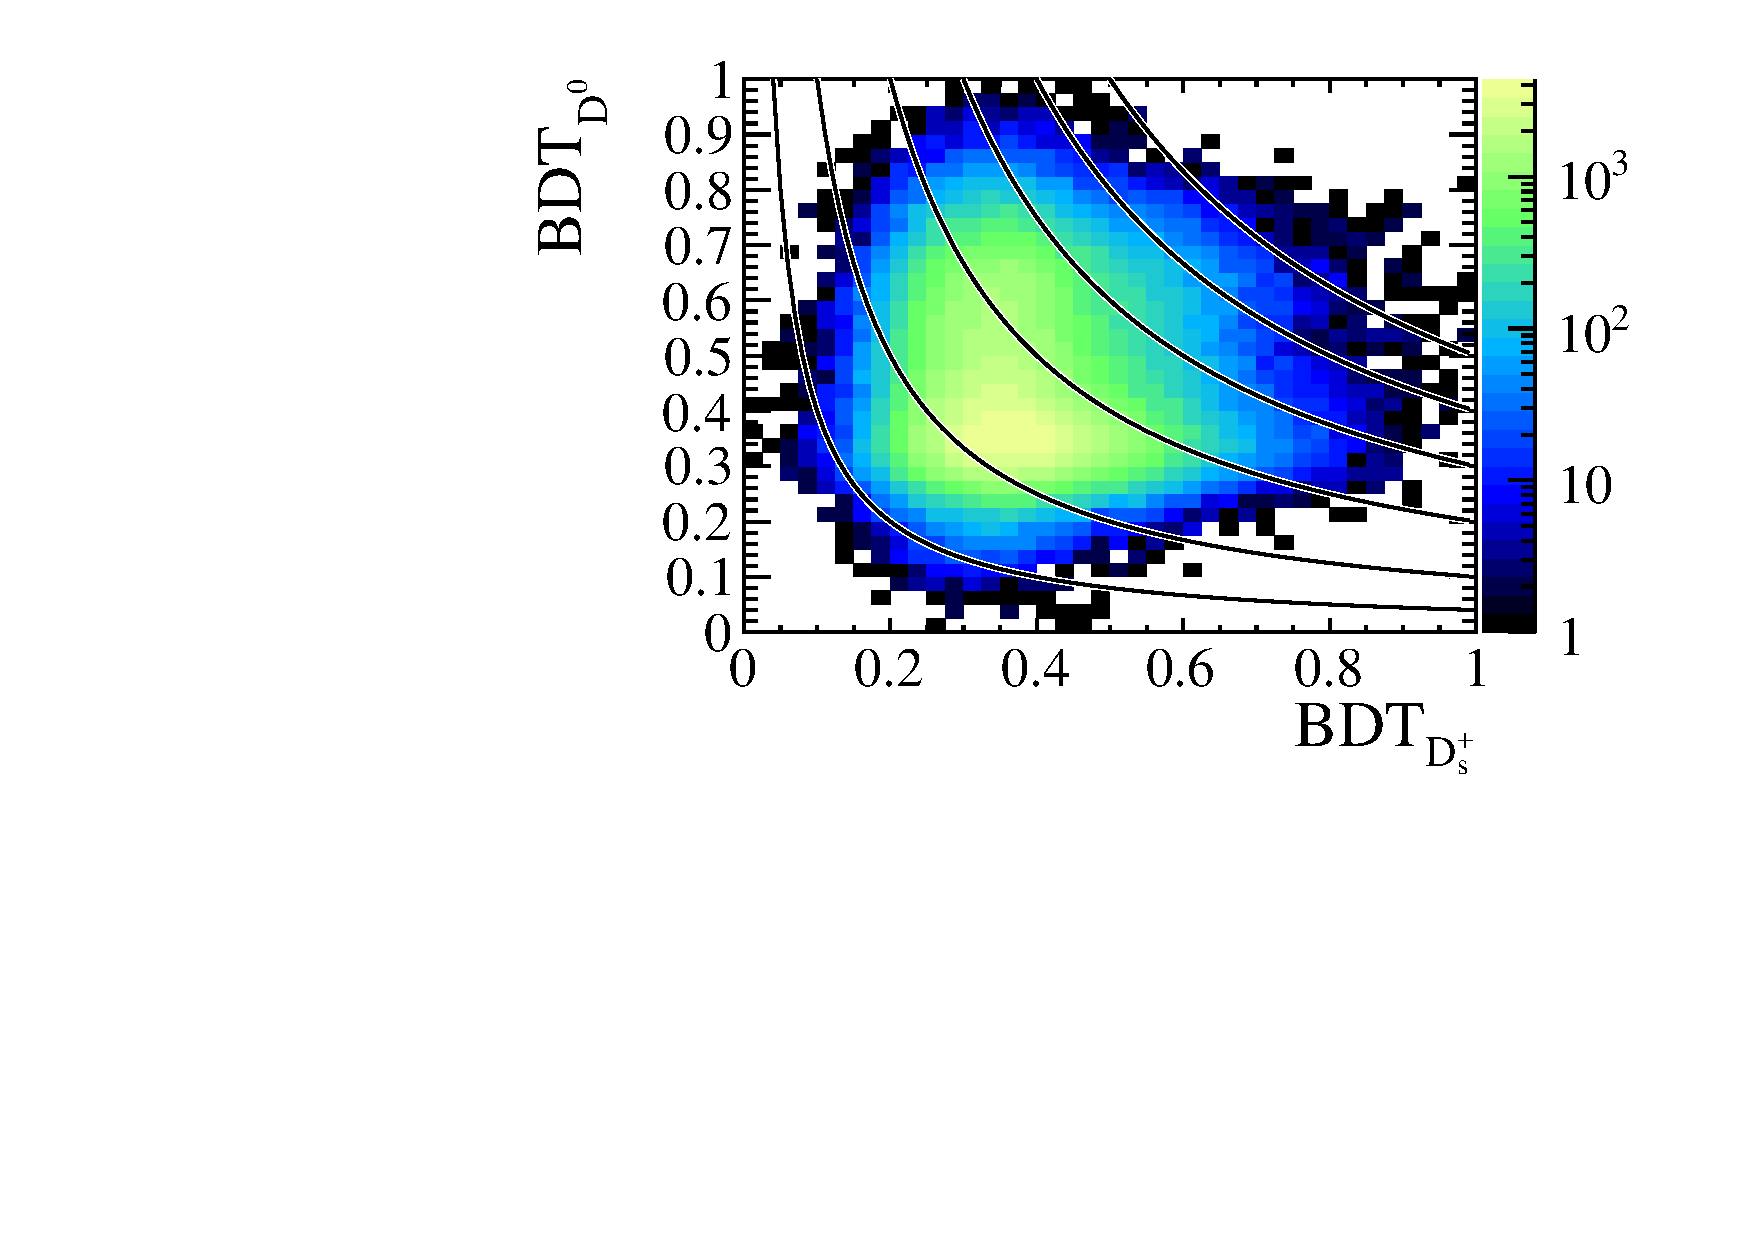
\includegraphics[width=0.48\textwidth]{dbdts}
    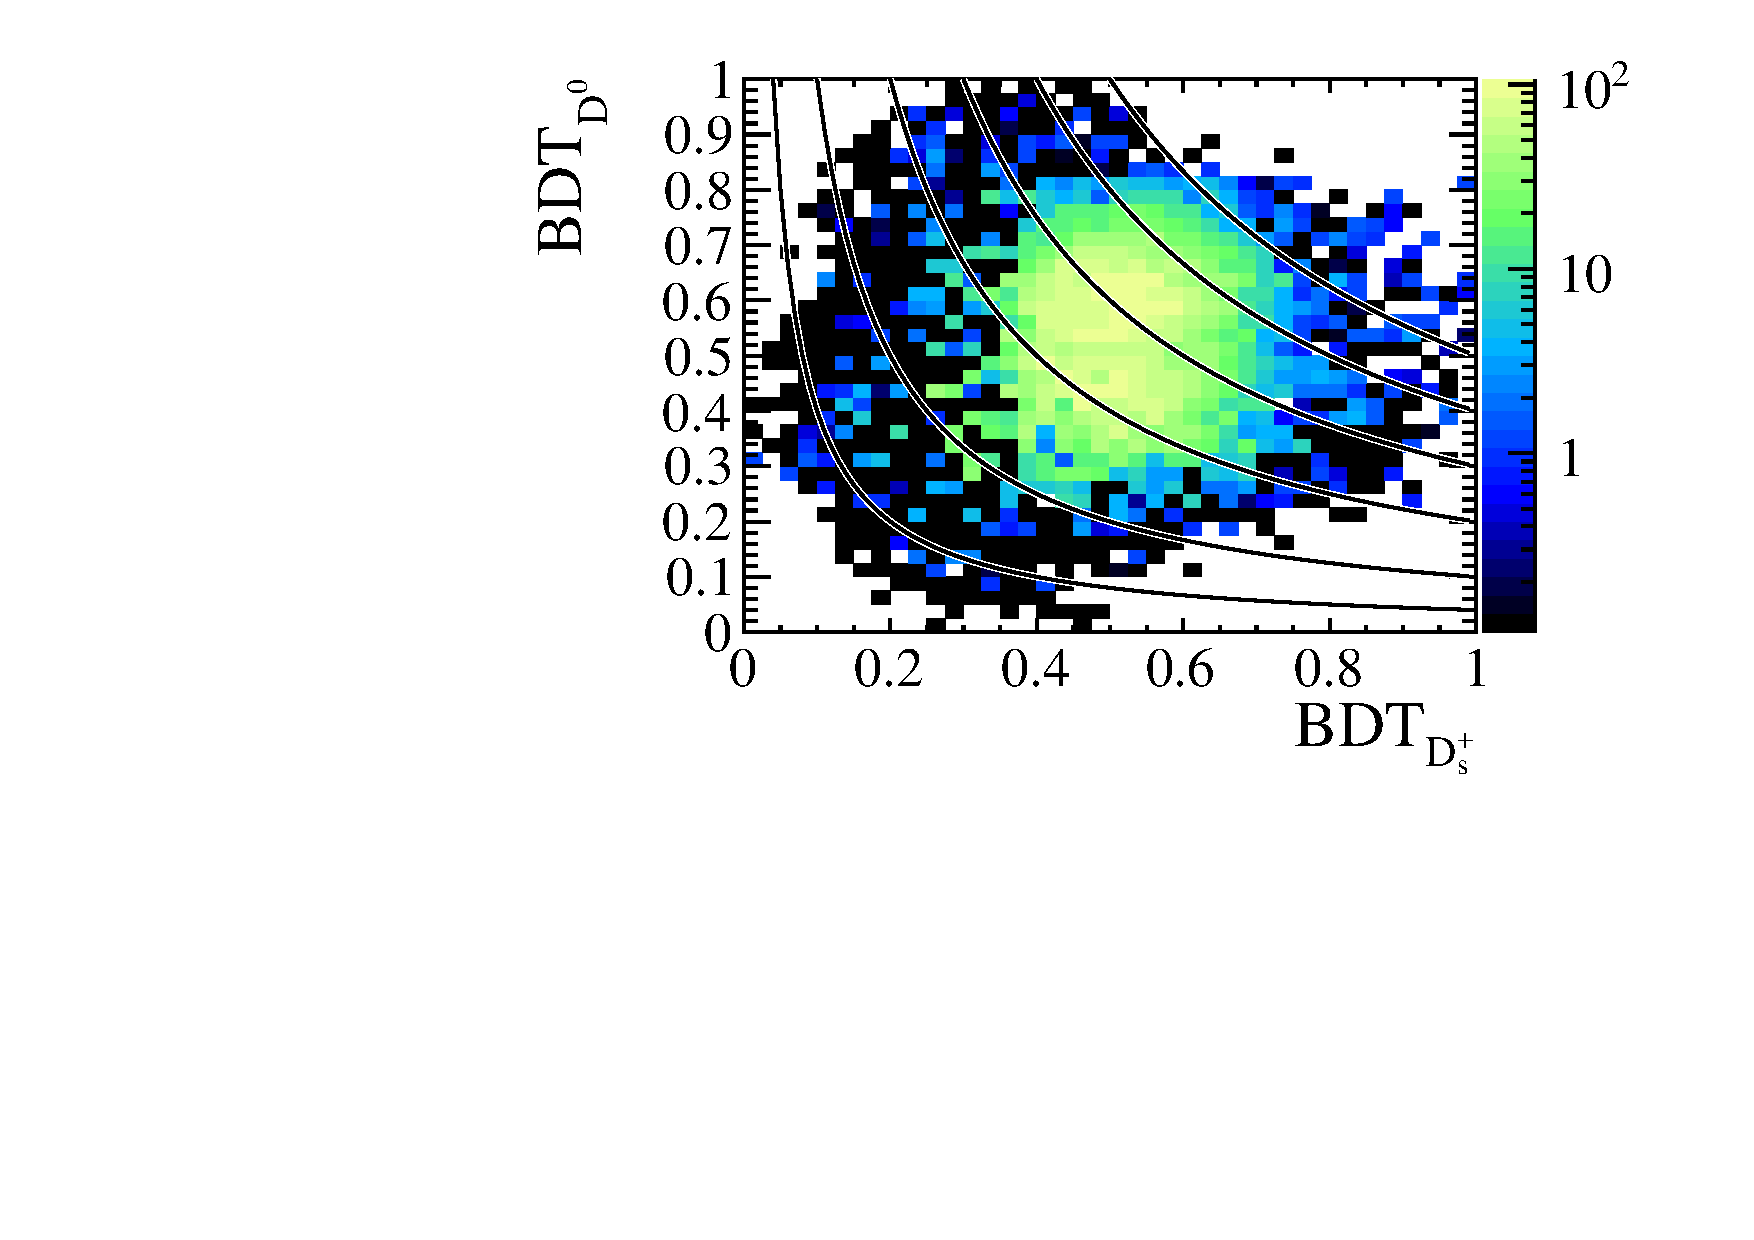
\includegraphics[width=0.48\textwidth]{dbdts_sw}
    \caption[Example distribution of $\mathrm{BDT}_{D_s^+}\times\mathrm{BDT}_{D^0}$ from candidates
      for the decay \btodsd]
    {
      An example distribution of the response for a $\bdt_{\Dz}$ against a $\bdt_{\Ds}$ for a
      sample of (left) \btodsd candidates where the background dominates and occupies the lower
      left of the plots, and (right) the same candidates after sWeighting has been applied where
      the signal peak is observed further towards the upper right.
      The lines overlayed on the plot are show the boundaries for the cuts of
      $\bdt_{\Ds}\times\bdt_{\Dz}>0.01$, 0.04, 0.10, 0.20, 0.30, 0.40, and 0.50.
      It is seen that using the product of the \bdt discriminants is more effective for rare decays
      where a tighter cut will be needed, in this region candidates are selected if their response
      is particularly positive, at the expense of the other meson.
    }
    \label{fig:dsphi:bdtprod}
  \end{center}
\end{figure}

%Each BDT was trained using the bagging method, as described in \Sec{sec:bdt:bag}.
%The signal and background data used to train these BDTs came entirely from data.
%Signal samples came from the decays $\decay{\Bbar^0_{s}{\Ds\pim}$ and $\decay{\Bs}{\jpsi\phi}$
%data, which was background subtracted by sWeighting~\cite{splot}.
%Background samples were taken from the sideband distributions of the same data.
%The BDT technique used in this analysis, also used in \Ref{LHCb-CONF-2012-009}, is different to
%other analyses in this thesis in that a BDT is trained for each the \Ds and $\phi$.

The \dstokkpi \bdt was trained using \dstokkpi decays from data taken from the
high statistics channel \decay{\Bsb}{\Dsp\pim}.
The signal sample of \Ds decays came from the \dstokkpi candidates that fell within $3\sigma$ of
the known \Ds mass, the sample was
background subtracted using the sWeighting technique~\cite{splot} on the \Bp mass spectrum.
Background data was taken from candidates falling in the upper mass sideband of the \Bp, and either
sideband of the \Ds.
Similarly, for the \phii\ \bdt, the signal sample was sWeighted and the background comes from the
\phii mass sidebands; but the sample is taken from the high statistics \bstojpsiphi mode.

%Considering that each \bdt was trained on data, variables that are poorly described in simulation
%can be used in the training.
In total, there are five kinematic and geometric training variables for the parent meson.
For the daughter tracks there are a total of 23 variables, including kinematic, geometric and \pid
variables.
Since the \bdt was trained using data, it is possible to use \pid variables that are poorly
described in simulation.
A summary of all training variables is given in \Tab{tab:dsphi:vars}.

%The BDT used to separate background from the signal \decay{\Ds}{\kkpi} decays was trained using
%a signal sample of \decay{\Bs}{\Dsm\pip} sWeighted~\cite{splot} data, and background from the \Dsm
%sidebands.
%This BDT uses an unusually large array of training variables, given in \Tab{tab:dsphi:vars},
%which include PID, and track quality variables.

\begin{table}
  \caption[BDT variables]
  {
    List of training variables used in the \Ds and \phii BDTs.
    Each BDT uses five variables associated with the parent particle and 23 variables from each
    daughter track.
  }
  \label{tab:dsphi:vars}
  \begin{center}
    %\begin{tabular}{clp{0.50\textwidth}}
    %\begin{tabular}{p{0.1\textwidth}p{0.3\textwidth}p{0.50\textwidth}}
    \begin{tabular*}{\textwidth}{ll @{\extracolsep{\fill}} p{0.6\textwidth}}
      \toprule
      Particle & \multicolumn{2}{c}{Variable} \\
      \midrule
      \Ds, \phii
      & Kinematic variables & $p$, \pt \\
      & Geometric variables & \chisqvtx, \chisqip, \chisqfd \\
      \littlerule
      Tracks
      & Kinematic variables & $p$, \pt \\
      & Geometric variables & $\min(\chisqip)$ \\
      & Track variables     & 4 variables characterizing the track quality \\
      & PID variables       & 16 variables containing PID information, such as {\tt isMuon} and DLL
      variables from the \rich detectors \\
      \bottomrule
    %\end{tabular}
    \end{tabular*}
  \end{center}
\end{table}


The cut for the \bdt was optimized using the metric $S/\sqrt{S+B}$,
In this case, the number of signal events, $S$, was estimated from the yield from the decay
\decay{\Bs}{\Dsm\pip}, according to:
\begin{equation}
  S = \frac{ \BF\big(\btodsphi\big) }{ \BF\big(\Bsb\!\to\Ds\pim\big) }
  \frac{ \eff{gen}\big(\btodsphi\big) }{ \eff{gen}\big(\Bsb\!\to\Ds\pim\big) }
  \frac{f_d}{f_s}
  N\big(\Bsb\!\to\Ds\pim\big),
\end{equation}
$f_s/f_d$ quantifies the fraction of \Bs mesons produced relative to \Bd mesons.
The generator level efficiency, \eff{gen}, is the efficiency introduced by the acceptance region of
the \lhcb detector, and the necessity that all daughter particles must travel through the detector.
Background yield for a given cut is estimated as:
\begin{equation}
  B = c\cdot N_\mathrm{c}\big(\bstodspi\big)\cdot N_\mathrm{c}\big(\bstojpsiphi\big),
\end{equation}
where $N_\mathrm{c}$ indicates the yield of the combinatoric background for the indicated decay,
and $c$ is a constant scaled such that $N_\mathrm{c}\big(\bstodspi\big)\cdot
N_\mathrm{c}\big(\bstojpsiphi\big)=N_\mathrm{c}\big(\btodsphi\big)$ with no \bdt cut.
The optimization procedure results in the optimal cut as $\bdt_{\Ds}\times\bdt_\phi>0.57$, as is
shown in \Fig{fig:dsphi:opt}.


\begin{figure}
  \begin{center}
    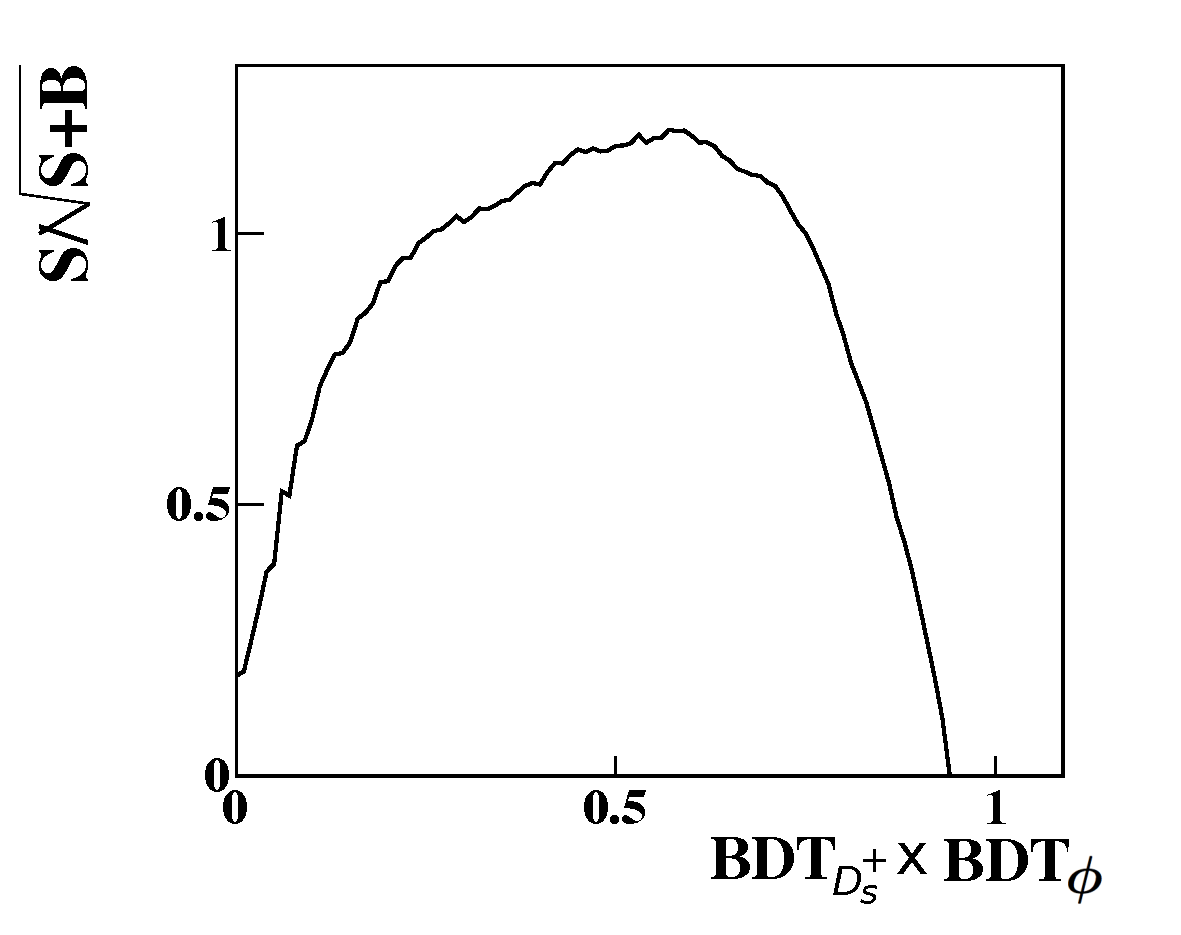
\includegraphics[width=0.48\textwidth]{dsphi_opt}
    \caption[Optimization of BDT cut for selection of \btodsphi candidates]
    {
      Value of the figure of merit $S/\sqrt{S+B}$ is shown as a function of the \bdt response,
      $\bdt_{\Ds}\times\bdt_{\phi}$.
      The maximum value of the figure of merit is 0.57, which is chosen as the final \bdt cut.
    }
    \label{fig:dsphi:opt}
  \end{center}
\end{figure}





\subsection[Vetoes of {\Dp} and {\Lc} deacys]
{Vetoes of $\boldsymbol{\Dp}$ and $\boldsymbol{\Lc}$ decays}
\label{sec:dsphi:sel:veto}
There are few backgrounds from real particles that could contaminate the final selection after the
\bdt selection.
The decay topology of \dstokkpi is very similar to the other weak decays \decay{\Dp}{\kpipiss} and
\decay{\Lc}{\pkpi}, which both
have relatively large branching fractions~\cite{PDG2012}:
\begin{align}
  \BF(\decay{\Dp}{\kpipiss}) &= (9.13\pm0.19)\e{-2}, \nonumber\\
  \intertext{and}
  \BF(\decay{\Lc}{\pkpi}) &= (5.0\pm1.3)\e{-2}.\nonumber
\end{align}
If the daughter $\pip(\proton)$ from the $\Dp(\Lc)$ decay is misidentified as a \Kp the decay
\dstokkpi can be mimicked.
%the resulting invariant mass combination can fall within $25\mev$ of \mass{\Ds}.
Henceforth, the notation $h_i$ will be used to denote a particle assigned the mass of an $h$ which
has been identified as an $i$.
Simple generator level simulations of phasespace, as shown in \Fig{fig:dsphi:veto}, illustrate that
the mass combination of $\Kp_\pi\Km\pip$ and $\Kp_p\Km\pip$ from a real \Dp or \Lc, respectively,
can fall within $25\mev$ of $\mass{\Ds}^\pdg$.


\begin{figure}
  \begin{center}
    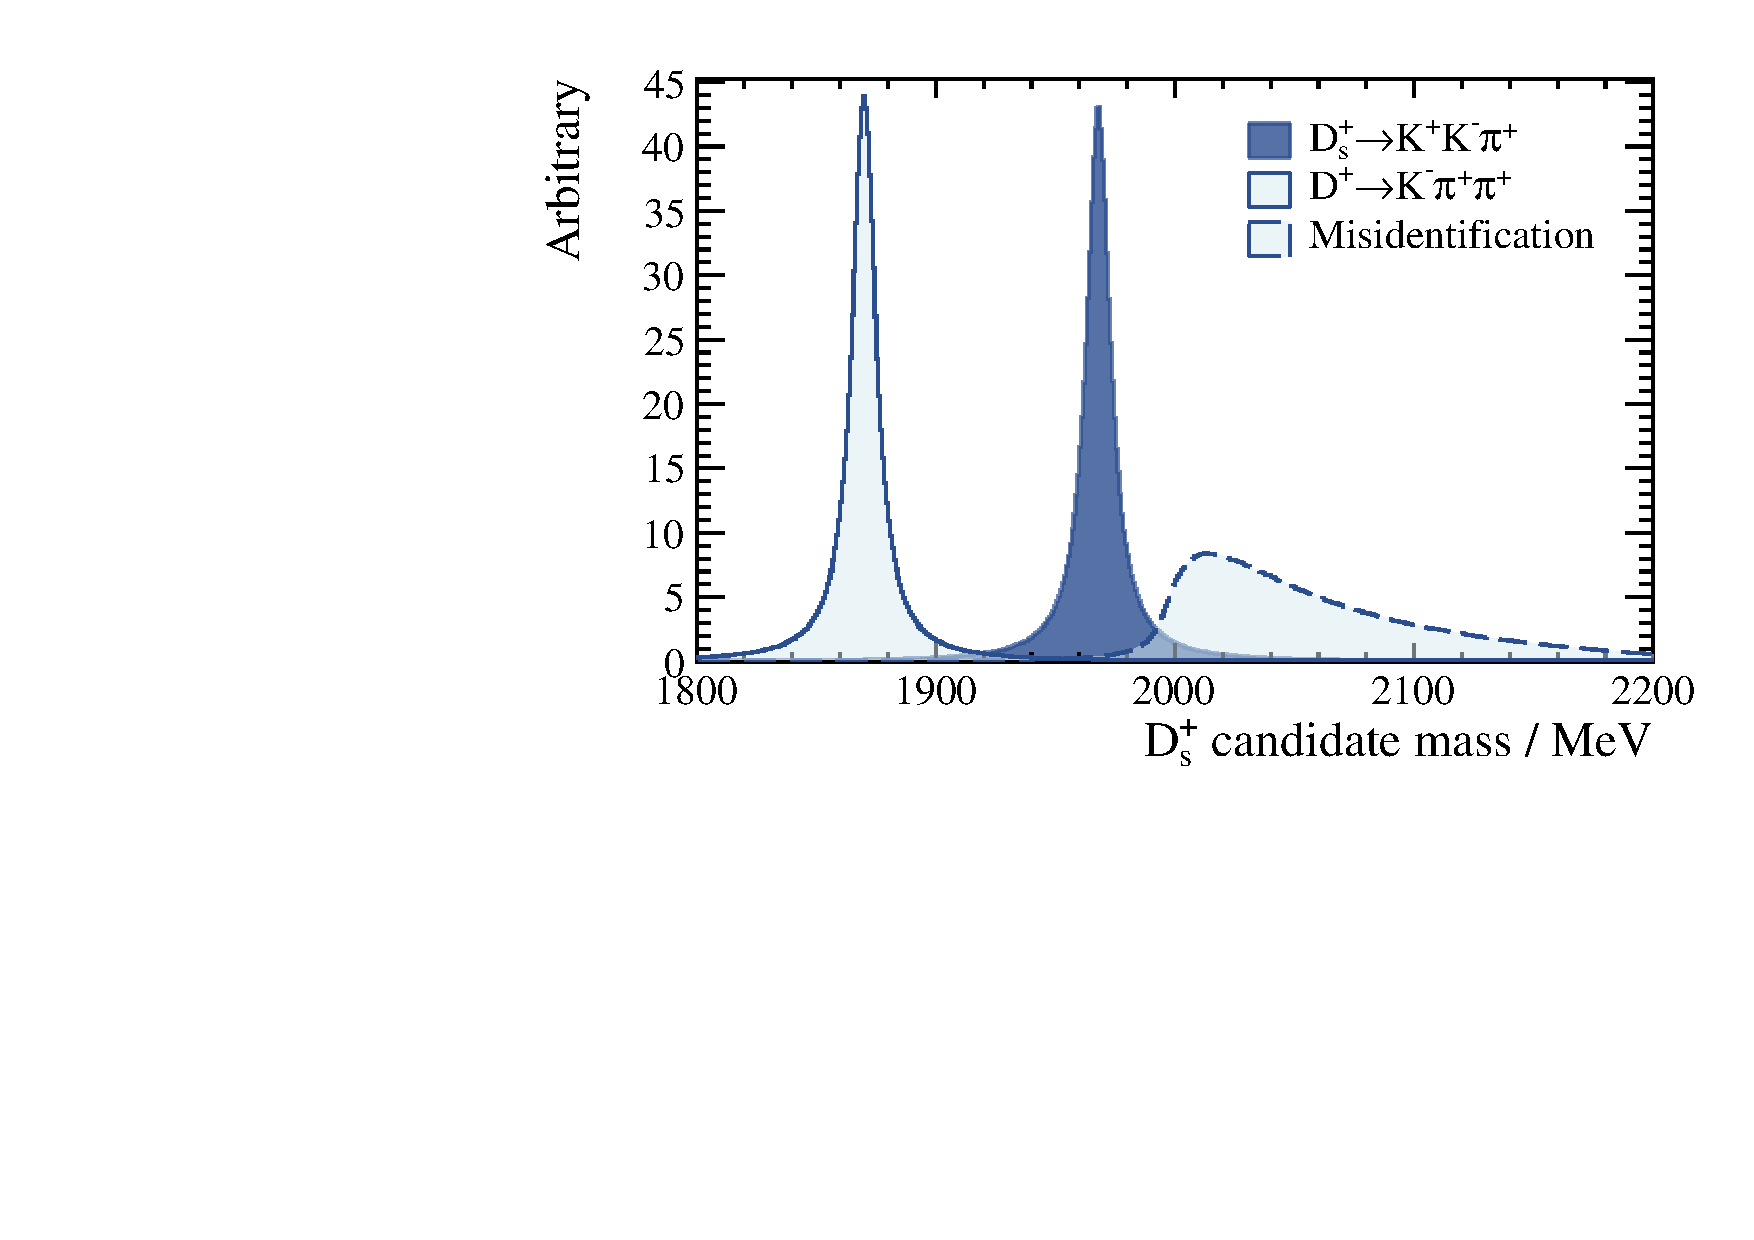
\includegraphics[width=0.48\textwidth]{tgen_dveto}
    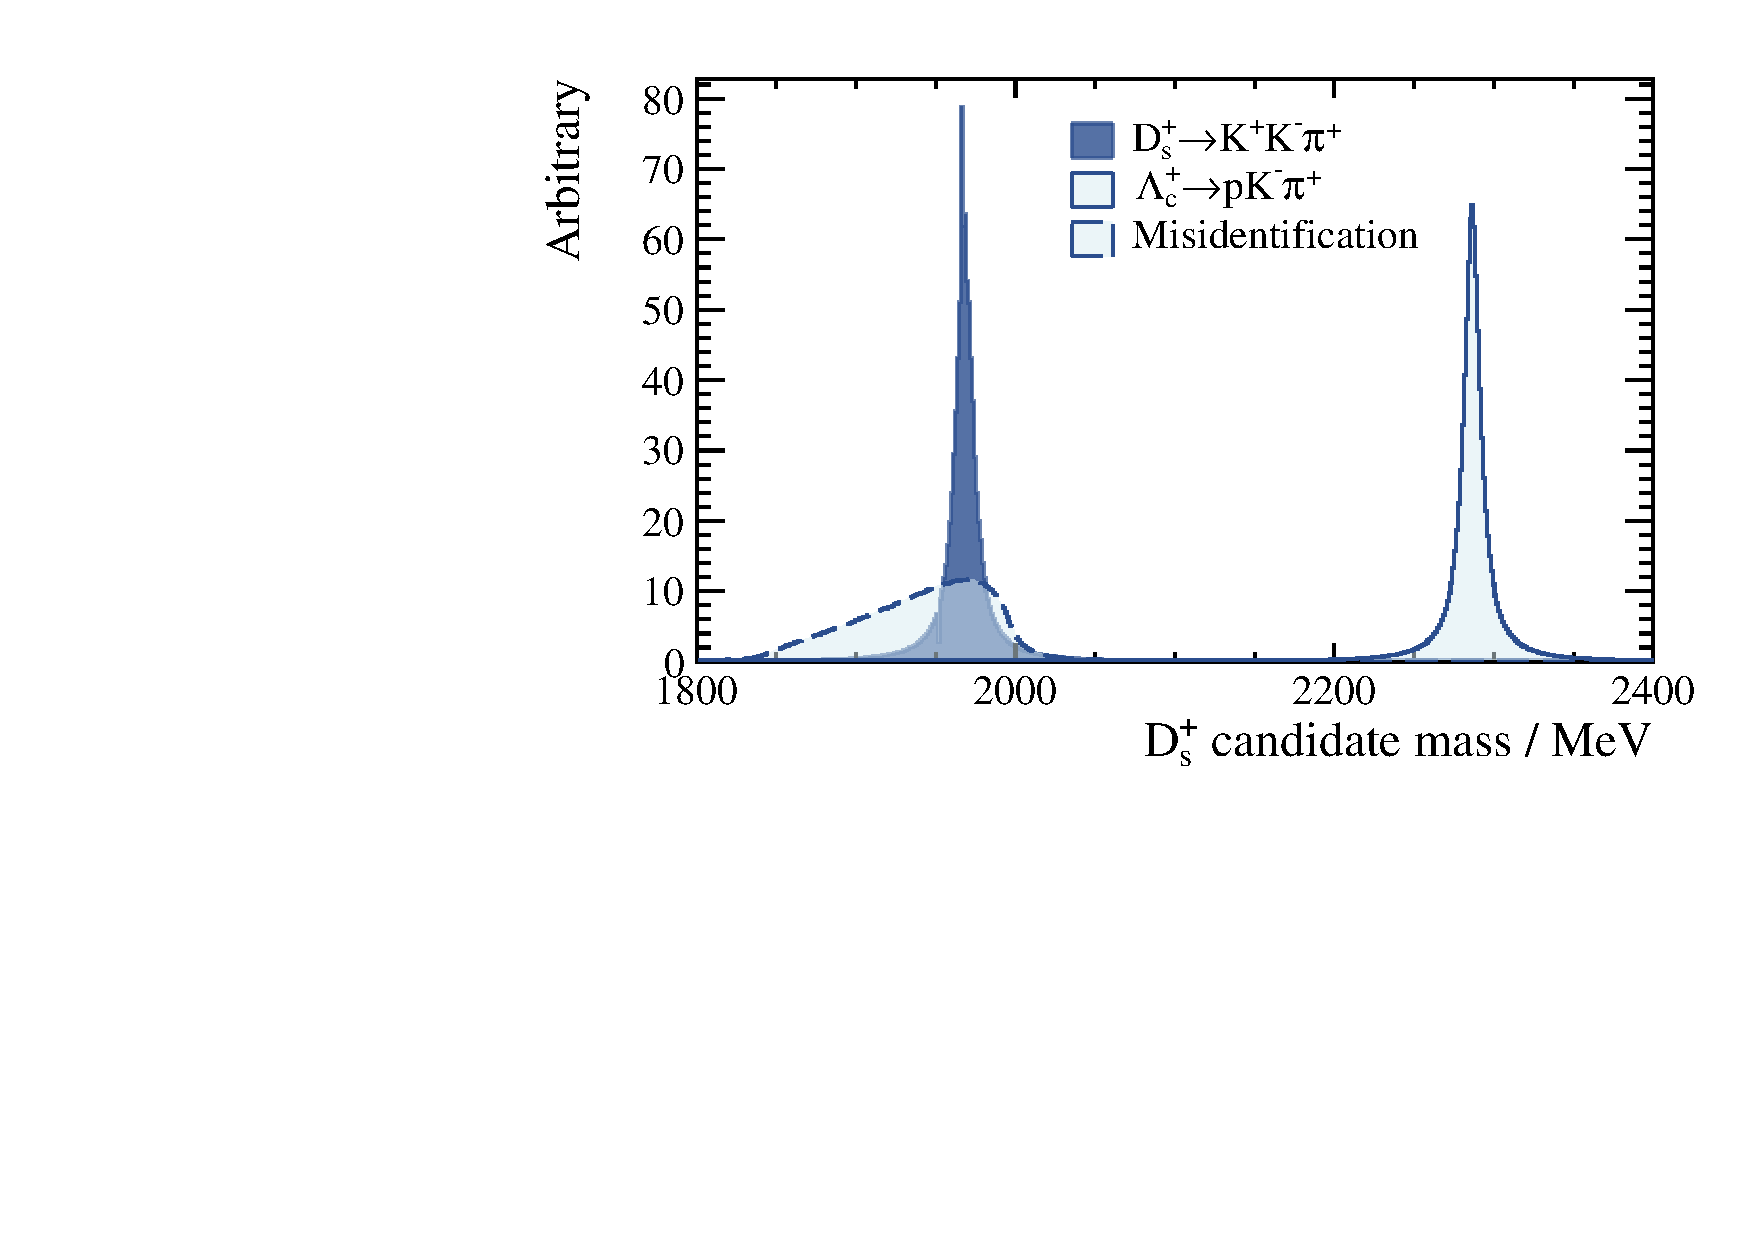
\includegraphics[width=0.48\textwidth]{tgen_lcveto}
    \caption[Vetoing \Ds contamination from \Lc and \Dp decays]
    {
      Simple phasespace simulations at generator level of the decay \decay{\Ds}{\kkpi}, along side
      (left) \decay{\Dp}{\kpipiss}, and
      (right) \decay{\Lc}{\pkpi},
      The distributions of the \Dp and \Lc decays, where one particle has been misidentified as a
      \Kp are also shown.
      Distributions after the misidentification are shown with a dotted outline, and sit under the
      \Ds mass peak.
      Magnitudes of each peak are meaningless, each having the same integral.
    }
    \label{fig:dsphi:veto}
  \end{center}
\end{figure}

The cross-feed from the \Dp and \Lc is suppressed by vetoes, whereby tight \pid constraints are
applied if the \dstokkpi candidate could have come from either a \Dp or \Lc.
Firstly, if the invariant mass of the \kk pair is lies within $10\mev$ of the nominal \phii mass
then it is highly likely that it is a real \Ds decaying via \decay{\Ds}{\phi\pip}, which has a
branching fraction of $(4.5\pm0.4)\e{-2}$ and therefore the \kkpi combination is immediately
accepted as a \Ds candidate.
Secondly, if the invariant mass of the $p_K\Km\pip(\Km\pip_K\pip)$ object falls within $25\mev$ of
the known $\Dp(\Lc)$ mass the ambiguous particle is subject to harsh \pid requirements, such that:
$\dllkpi>10(\dllkp>0$).
These vetoes are highly, \approx$95\pc$, efficient.



%There is potential for cross-feed from the decay \decay{\Dp}{\kpipiss} and
%the signal \Ds final state if one of the \pip{s} is misidentified as a \Kp.
%The resulting invariant \kkpi combination --- with one kaon being a misidentified pion --- may fall
%within $25\mev$ of the nominal \Ds mass.
%%This is possible because the \Ds is approximately $100\mev$ heavier than the \Dp.
%Similarly, there is potential contamination from the decay \decay{\Lc}{p\Km\pip}.
%These two modes of cross-feeds are suppressed by a series of conditions.
%Firstly, if the mass of the \kk pair from the \Ds decay is within $10\mev$ of the \phii mass, then
%the candidate is accepted as coming from the decay \decay{\Ds}{\kkpi}.
%Otherwise, a track is assigned the mass of a pion or proton, so as the new object is consistent
%with a \kkpi or $p\Km\pip$, respectively.
%If the invariant mass of this newly reconstructed object falls within the nominal mass of the \Dp
%or \Lc, then the ambiguous (swapped) track is subject to the stringent PID requirements of
%$\dllkpi>10$ or $\dllkp>0$, respectively.



Invariant mass distributions of
selected candidate \Ds and \phii mesons after the selection are shown in \Fig{fig:dsphi:mesons}.

\begin{figure}
  \begin{center}
    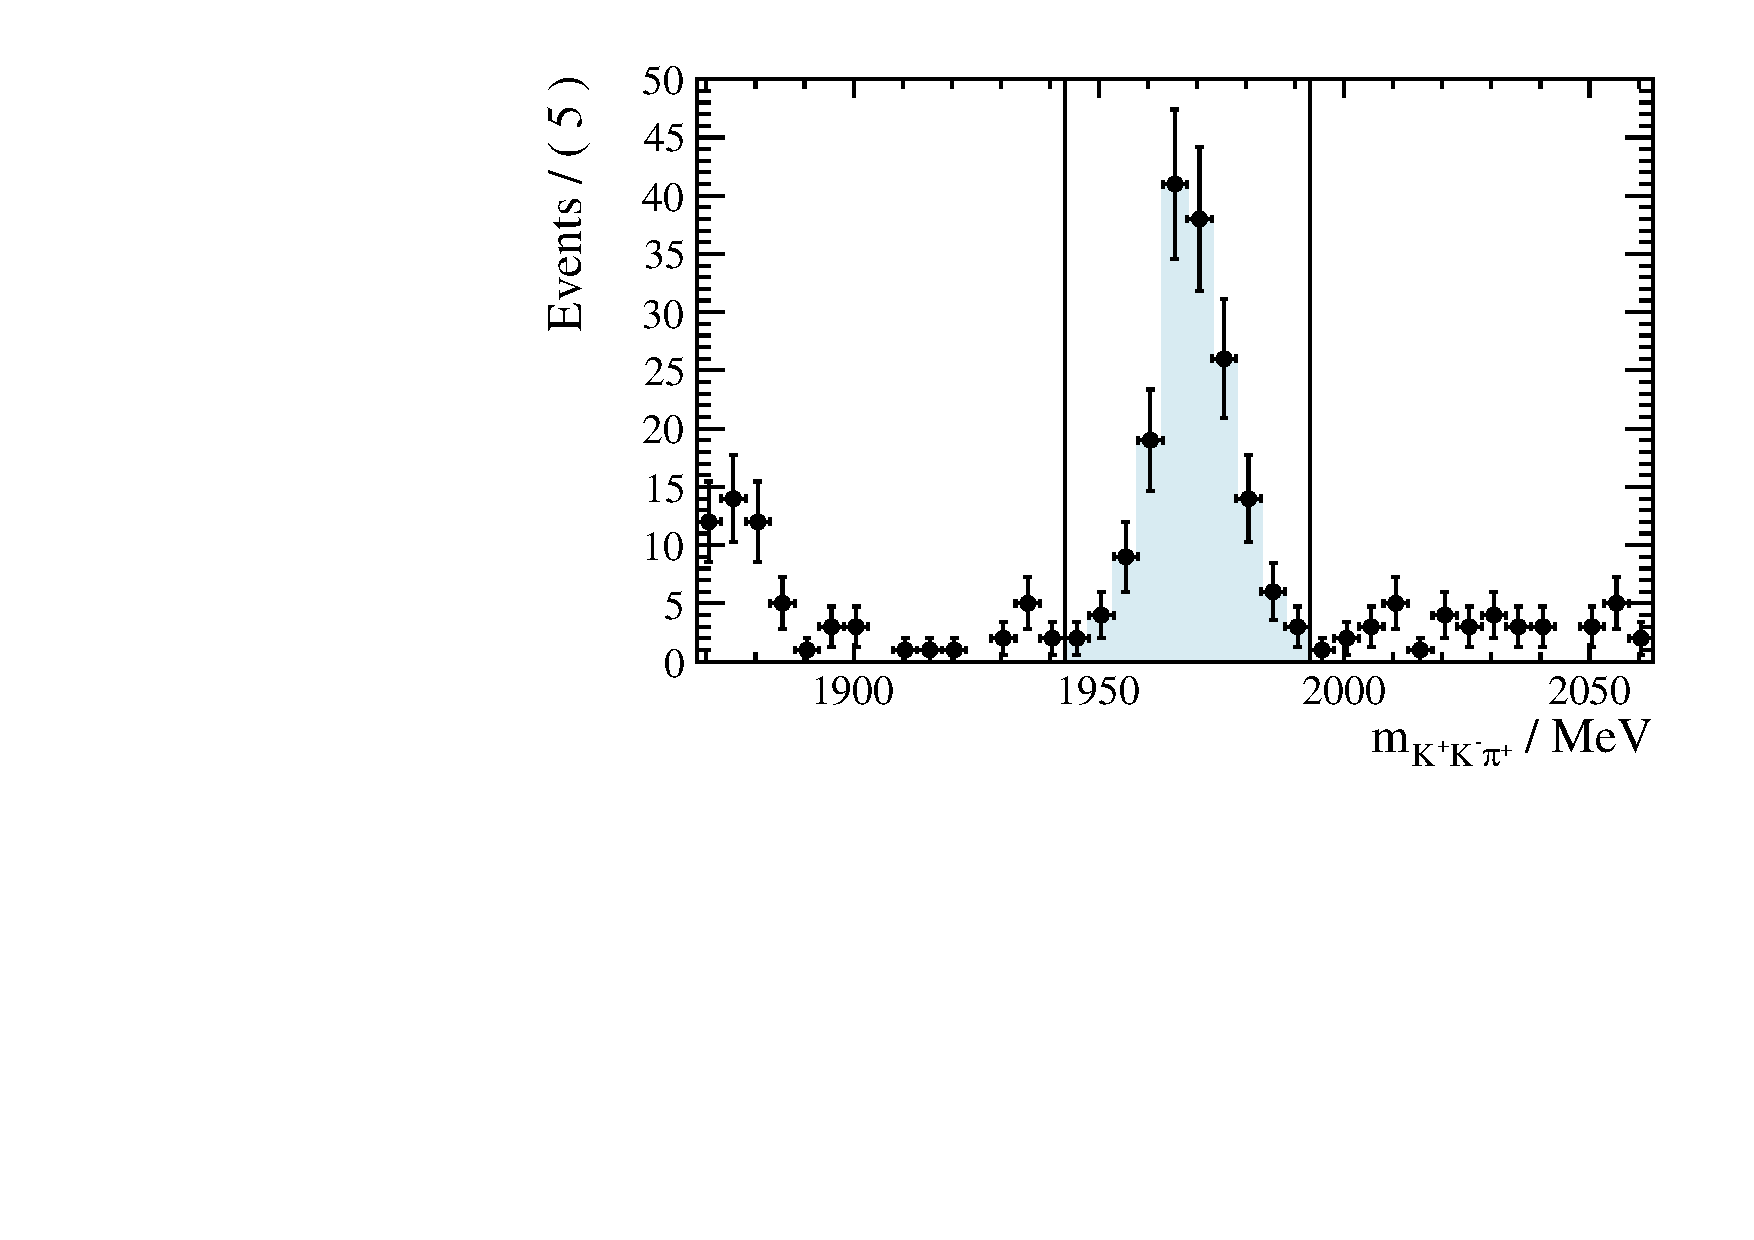
\includegraphics[width=0.48\textwidth]{spectrum_ds}
    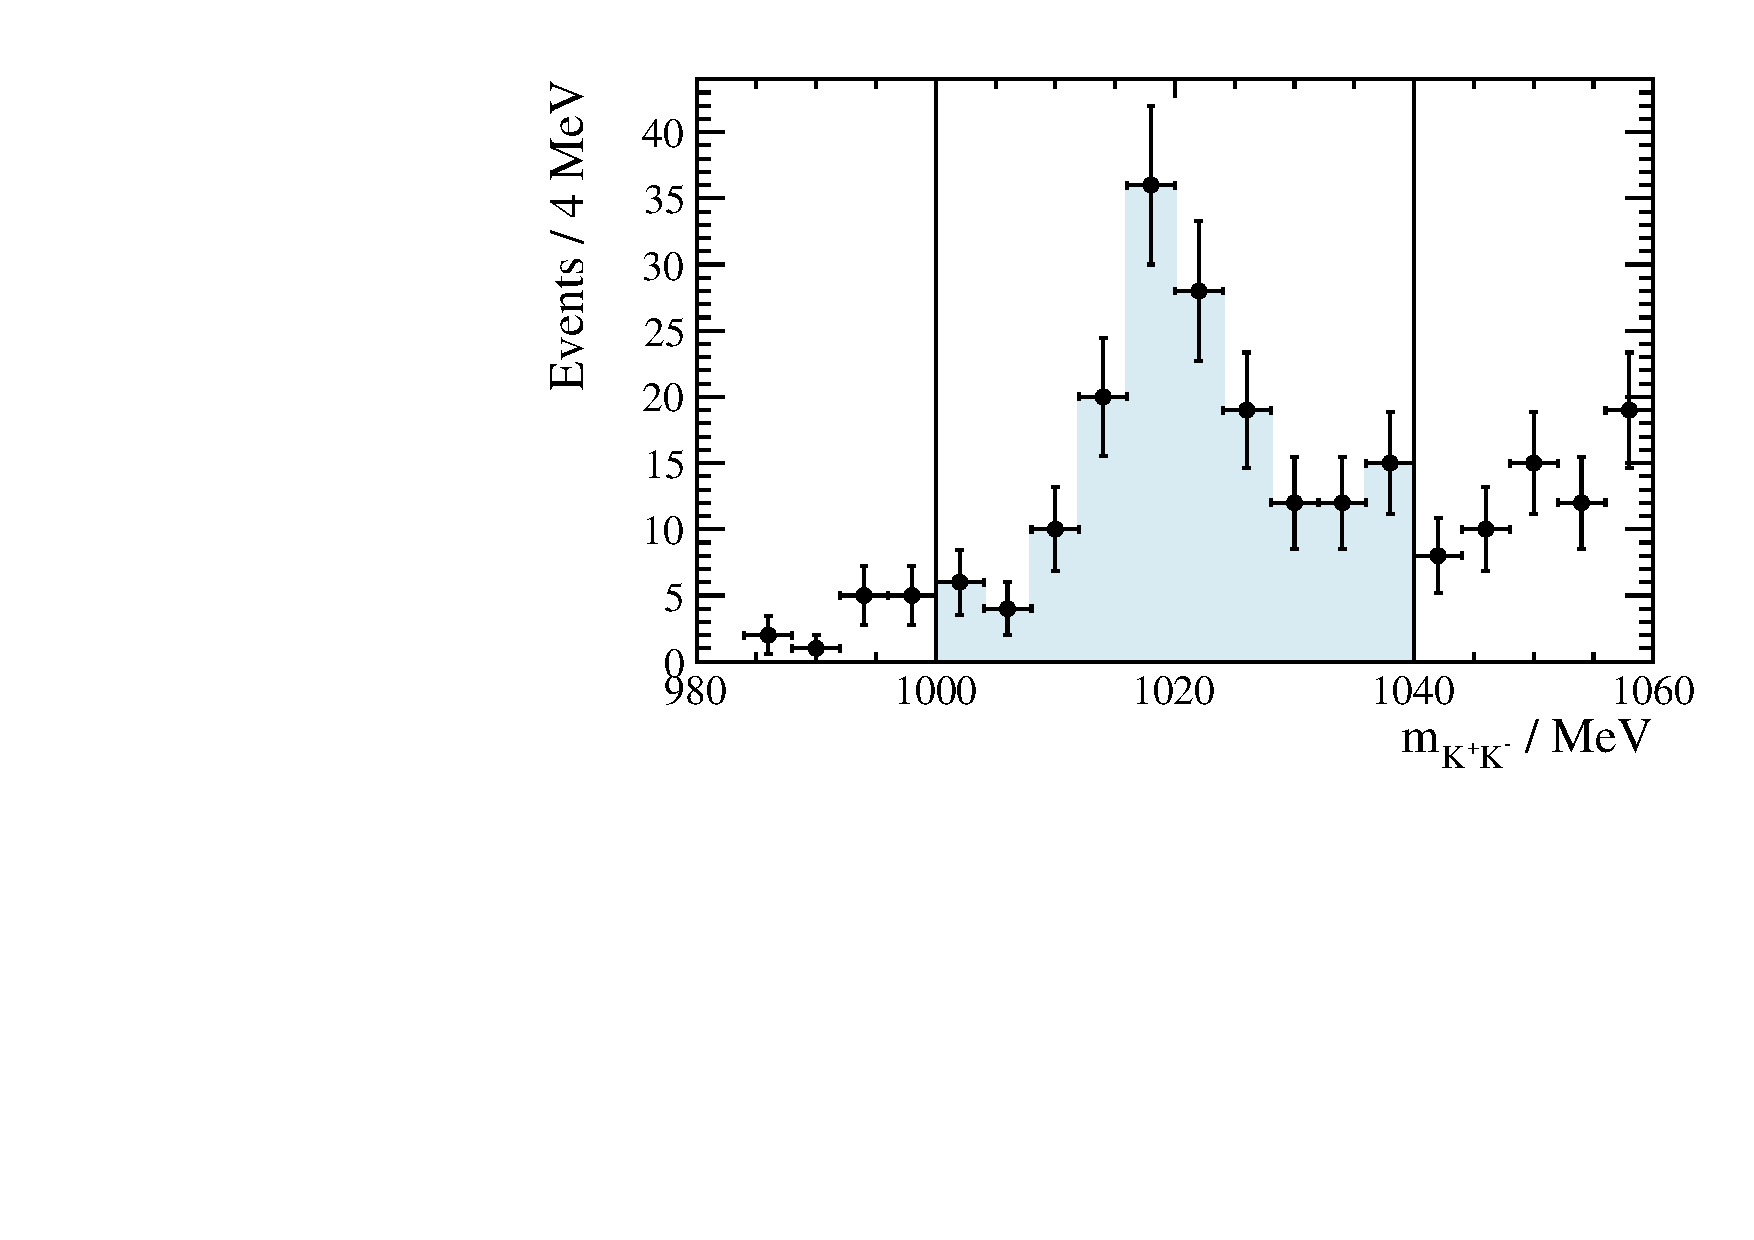
\includegraphics[width=0.48\textwidth]{spectrum_phi}
    \caption[Selected \Ds and \phii candidates]
    {
      Invariant mass distributions of the candidate
      (left) \decay{\Ds}{\kkpi}, and
      (right) \decay{\phii}{\kk} candidates.
      The \kkpi spectrum shows a range of masses, where the vertical black lines indicate the
      boundaries of the mass cut $|m_{\kkpi}-m_{\Ds}^\pdg|<25\mev$, where the shaded candidates are
      those that are accepted.
      On the far left of this distribution, a mass peak from \decay{\Dp}{\kkpi} is also visible.
      The \decay{\phi}{\kk} spectrum is shown in the range $|m_{\kk}-m_{\phi}^\pdg|<40\mev$,
      and the signal region is indicated by the vertical black lines and shaded data.
    }
    \label{fig:dsphi:mesons}
  \end{center}
\end{figure}

